\documentclass[english, 12pt]{scrartcl}
\usepackage{caladea}
%\usepackage{gfsartemisia-euler}
\usepackage[
a4paper,
left=2.5cm,
right=2.5cm,
top= 2cm,
bottom = 2.5cm,
footskip = 1.5cm
]{geometry}
\usepackage{fancyhdr}
\usepackage[english]{babel}
\usepackage[T1]{fontenc}
\usepackage{graphicx,float}
\graphicspath{ {./images/} }
\usepackage{wrapfig}
\usepackage{caption}
\usepackage{pdfpages}
\usepackage{makecell}
\usepackage{subfiles}
\usepackage{enumitem,amssymb}
\usepackage{lastpage}
%\usepackage{amsmath}
\usepackage{esint}
\usepackage{blindtext}
\usepackage{hyperref}
\hypersetup{
	colorlinks=true,
	linkcolor=black,
	filecolor=magenta,      
	urlcolor=cyan,
	pdftitle={The Macruwu},
	pdfpagemode=FullScreen,
}
\urlstyle{same}
\usepackage[inkscapeformat=png]{svg}
\usepackage{tikz}
\usetikzlibrary{shapes.geometric, arrows}
\usepackage[
% school,
simplified
]{pgf-umlcd}
\usepackage{listings}
\usepackage{color}
\definecolor{listinggray}{gray}{0.92}





\pagestyle{fancy}

\title{\fontfamily{}\selectfont The Macruwu}
\author{Bramble}
\date{}
\begin{document}
	\maketitle
	\includegraphics[width=0.9\textwidth]{Macruwu PCB_5}
	\tableofcontents
	\newpage
	\section{Incentive}
	My handwriting is something any doctor would be proud of. My teachers, however, were not so enamoured with my writing prowess, often deducting grades for sheer illegibility. So when I went to uni, I started taking notes digitally. First, I tried my luck with OneNote and a digital pen, hoping somehow it would improve my notetaking-ability. But when that inevitably failed, I switched to Word. For those who have never tried, writing equations in Word is a pain in the back side. It takes ages and especially when equations get more complex, it's a nightmare to try and get the $e^{x}$ to go, where you want it to go.\\
	So I switched once more.I went for Markdown with inline $L^AT_EX$. Markdown is a markup language that can easily run in a browser and like $L^AT_EX$ it's "what you mean is what you get". It has simple syntax, making it easy to learn, but also supports inline $L^AT_EX$, which is very useful when writing equations. The hoster we (my friends and I) use also supports multiple people working on the same document in real time, which makes taking notes a lot faster and also allows one person to be sketching graphs and the like, while the rest of us try our best to keep up with the professor.\\
	But even with Markdown and multiple people writing at the same time, it just took too long and we sometimes missed some important notes.\\

	\begin{wrapfigure}{r}{0.25\textwidth}
		\vspace{-0.8cm}
		\centering
		\includegraphics[width=0.25\textwidth]{Macropad 0-1}
		\caption{Macropad v0.1}
	\end{wrapfigure}
	\noindent One afternoon I therefore cobbled together my first macro pad out of some Cherry switches and a Teensy I had lying around. It was extremely botched and had no fancy features to speak of, but it worked. That got me hooked. Even with just eight extra keys, I was able to write a lot faster. So I went back to the drawing board and started designing what was to become the Macruwu.
	\section{Requirements}
	For this macropad to be of any use to me, it needed to fulfil certain requirements.
	\begin{itemize}
		\item It needed to be compatible with any system. This meant it needed to work, no matter which computer I plugged it in to. This also meant that I couldn't rely on any software that had to be running in the background.
		\item It should be able to type out any key combination that would also be possible on a normal keyboard. This would make it universally useable for practically any software, because almost all software can be controlled easily with shortcuts from a keyboard.
		\item It must not hinder my workflow. This means that using the Macruwu should always be faster than typing out the command or character strings by hand.
		\item It needed to be fast. I wanted as little delay as possible, so that long strings of characters could be printed quickly. For complex equation presets a maximum delay of about 300-400ms would be optimal.
		\item Mappings should be changeable on the fly. If, for example, a certain equation were to show up consistently in the lecture, it should be possible to assign that equation to a key quickly and easily.
		\item It should be expandable. If 32 keys aren't enough or if I want to add some kind of other interface device or expansion module, it should be possible to interface it with the Macruwu.
		\item It MUST have RGB. I could try and think up some reason for why it's necessary to have RGB, but I just want RGB uwu.
		\item It should be affordable. The goal for this project was to stay under 70€ per unit.
		\item It should be repairable. For me this meant, creating options for most kinds of mechanical keyswitches. If a switch breaks or if I want to later replace them with different ones, it should be easy to just rip´em out and stick in some ones.
	\end{itemize}
	\newpage
	\section{Choices of component}
	\subsection{Microcontroller}
	For the microcontroller, I chose the seeed studio RP2040. It´s a small board, even smaller, than a Teensy, but it allows you to configure it as an HID with very little effort. It's also very fast and has a humongous 2MB of flash, which can also be configured as a mountable flash drive. It doesn't have a lot of pins but it does have a number of broken out connections, namely two I$^2$C lines, an SPI bus and even a UART port if you need it. And USB-C is just the cherry on top (no pun intended).\newline
	If you want to learn more, you can check out the \href{https://wiki.seeedstudio.com/XIAO-RP2040/}{Seeed Wiki}. This is good to get you started with the microcontroller, but if you want more information on the programming side, you should check out Earle Philhowers Arduino Pico \href{https://github.com/earlephilhower/arduino-pico}{GitHub} and \href{https://arduino-pico.readthedocs.io/en/latest/}{documentation}.
	
	\subsection{I/O expanders}
	In order to read the keyswitch inputs some kind of I/O expander was needed. I just went for the cheapest I could find on Mouser that was still in stock. It turned out to be the \href{https://www.mouser.de/datasheet/2/302/PCA9555-1127545.pdf}{PCA9555D}, a double 8-bit I/O expander that can be read via I$^2$C. It offers internal pull-up resistors, which was a nice bonus, meaning I didn't have to add them to the design. However, bear in mind that you might have to add some to your design if you want to use a different I/O expander.
	
	\subsection{Level shifter}
	The RP2040 is a 3.3V microcontroller. In order to use 5V logic devices, a level shifter is needed. This is optional, however. If you don't plan on using the NeoPixels or 5V I$^2$C devices, you can just leave it out. At first I used the \href{https://www.ti.com/lit/gpn/txu0104}{TXU0104PWR} which is a unidirectional chip. This works great for the NeoPixels, but won't work for the 5V I$^2$C due to this being a bidirectional protocol. However Texas Instruments offers a pin-equivalent bi-directional chip, the \href{https://www.ti.com/lit/gpn/lsf0204-q1}{LSF0204-Q1}. I haven't tested it so far, but the datasheet indicates that this should be a drop-in replacement.
	
	\subsection{RGB goodness}
	In order to satisfy my endless need for funny blinky lights, I picked up some \href{https://de.aliexpress.com/item/1005003636607308.html?spm=a2g0o.order_list.order_list_main.23.22bf5c5fJNwVec&gatewayAdapt=glo2deu}{SK6803 MINI-Es} from AliExpress. They come in 3mA and 12mA versions. In order to not overtax the USB power, I'd recommend getting the 3mA version. They should be more than bright enough. If you want to burn out your retinas, you can also go for the 12mA version, but bear in mind that you may run into Voltage drops when running them at the full 12mA.\newline
	One of the most useful features of the SK6803 MINI-Es is their ability to be mounted through a cutout in the PCB, making them sit flush with the surface. This allows the use of most switches. They also have a identical addressing scheme to standard NeoPixels and can be controlled by the Adafruit Neopixel library.
	
	\subsection{Hot-swap sockets}
	In order to change keyswitches without having to solder, some sort of hot-swap socket is needed. I chose \href{https://keycapsss.com/keyboard-parts/parts/49/kailh-hotswap-pcb-sockets-10-pcs?c=11}{Kailh hot-swap sockets}. They're easy to solder and work a lot better than the push-in ones you might find on commercial hot-swap boards. They also come in versions for MX- and Choc-style keyswitches.
	
	\subsection{Keyswitches}
	This is pure preference. I love clicky keys, so I went for the clickiest (reasonably priced) keys I could find. The \href{https://de.aliexpress.com/item/32980039972.html}{Gateron greens} are a very affordable option for MX style keys and are quite clicky. If you want maximum click for a bit more cash, you can check out the \href{https://keycapsss.com/switchestester/switches/65/kailh-low-profile-choc-switches?c=9}{Kailh whites}. They provide maximum click and are guaranteed to annoy the living heck out of most sane people. Needless to say I absolutely love them.\newline
	If you prefer not to make everyone within a 30Km radius go completely insane, you can also choose a tactile or linear switch. Both the Gateron and Kailh keys offer those options. If you want to fall in to a very deep rabbit hole, you can also look up keyswitches on YouTube. Trust me, it's worth it.
	
	\subsection{Keycaps}
	Now here there are several options. You can 3D-print your keycaps on a resin printer or print flat ones on an FDM printer and label them afterwards. You can get quite creative with custom keycaps. If you don't want to print your own, \href{https://de.aliexpress.com/item/1005003047698548.html}{relegendable keycaps} are always an option and the one I went for. A printable template for the keycap inlays is in the main GitHub repository.
	
	\subsection{I$^2$C Jacks}
	To connect the Macruwu to other input devices I used a \href{https://keycapsss.com/keyboard-parts/parts/54/2x-trrs-jacks-3.5mm?c=11}{3.5mm 4-pin headphone jack}. This breaks out 3.3V, GND, SCL, SDA and offers the option to use a wide variety of fancy cables.
	\newpage
	\section{Hardware}
	
	\subsection{Full schematics}
	\begin{figure}[H]
		\centering
		\includegraphics[width=0.9\textwidth]{sheet_1}
		\caption{Sheet 1 of the Macruwu}
	\end{figure}
	\begin{figure}[H]
		\centering
		\includegraphics[width=0.9\textwidth]{sheet_2}
		\caption{Sheet 2 of the Macruwu}
	\end{figure}
	\begin{figure}[H]
		\centering
		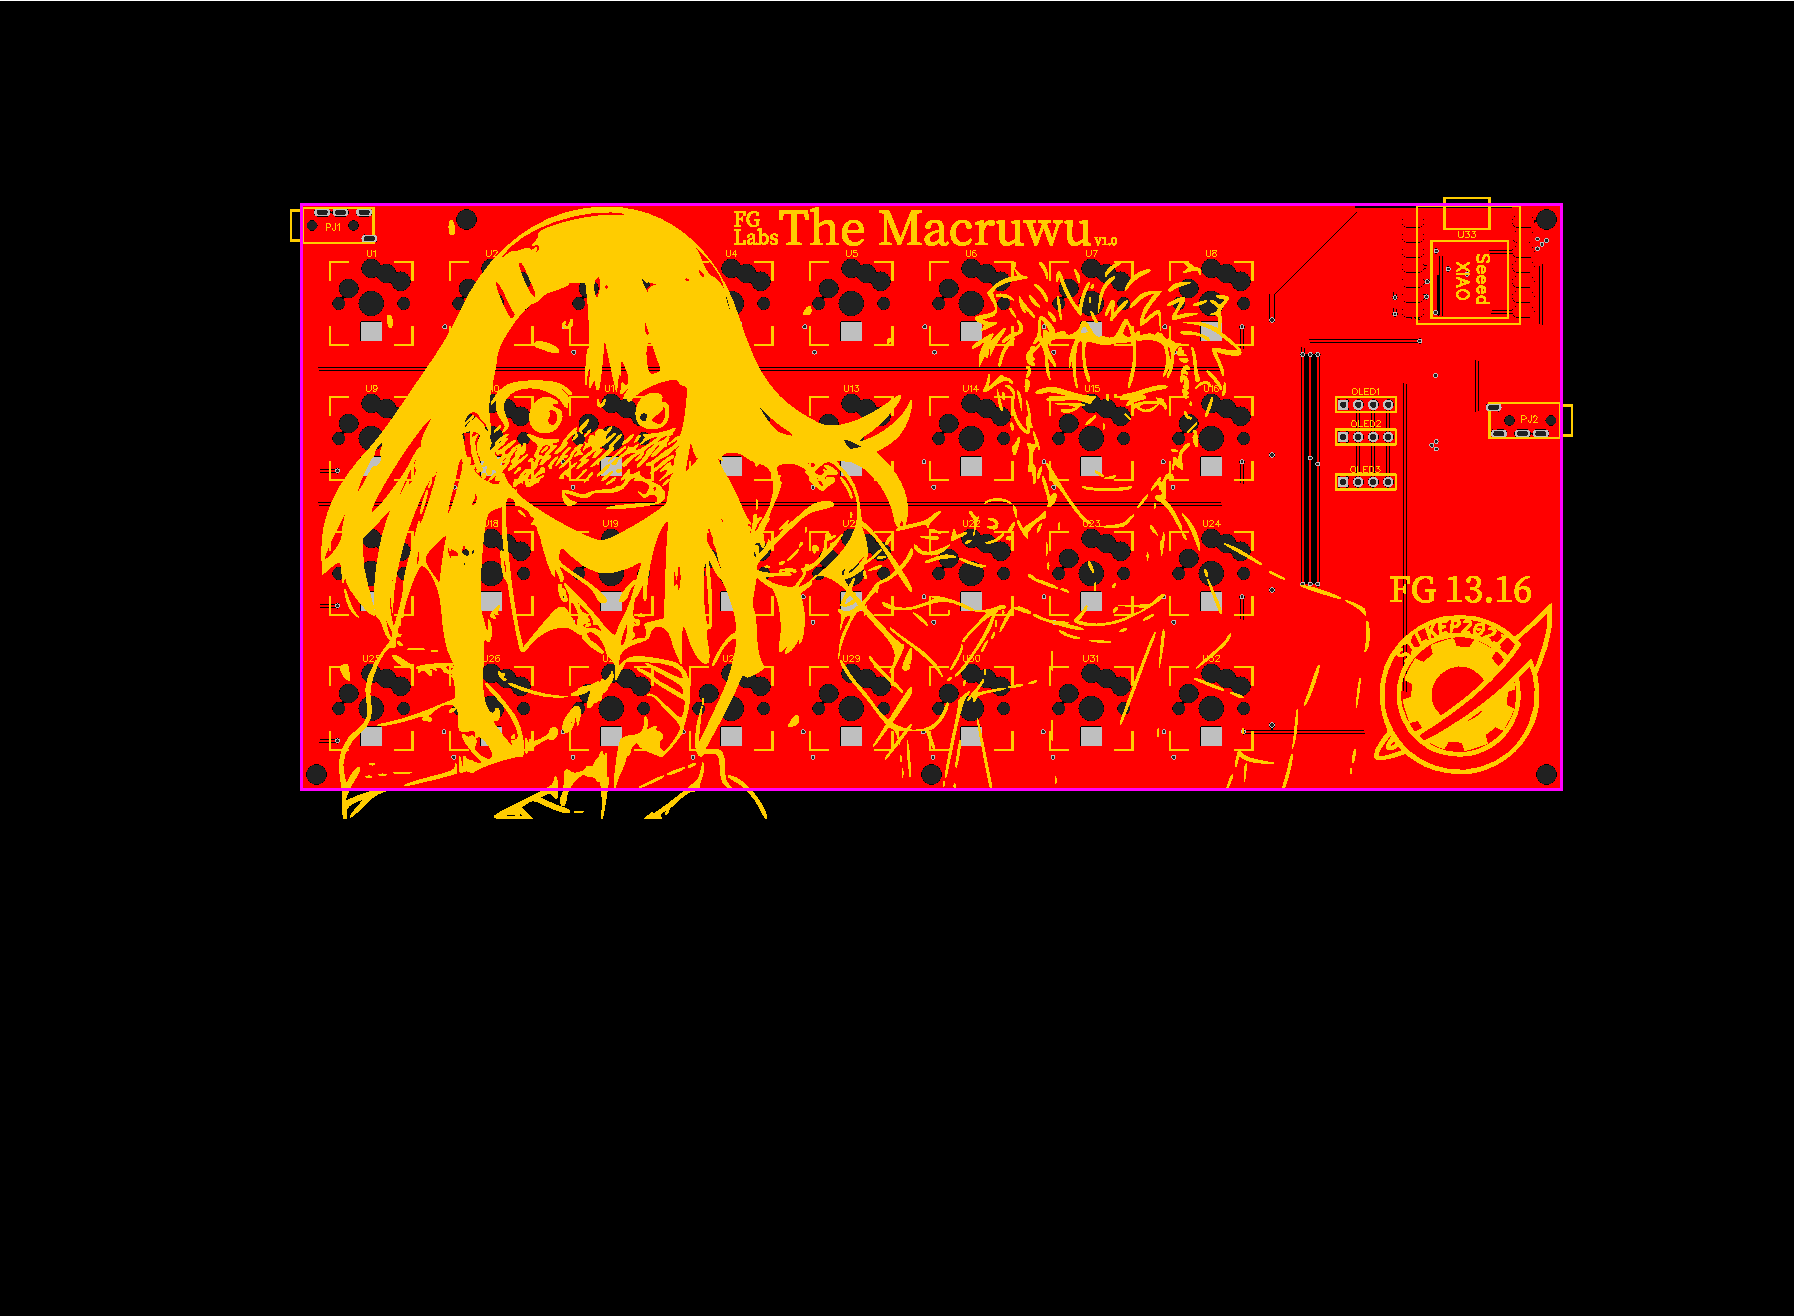
\includegraphics[width=0.9\textwidth]{Macruwu PCB_1}
		\caption{PCB frame 1 of the Macruwu}
	\end{figure}
	\begin{figure}[H]
		\centering
		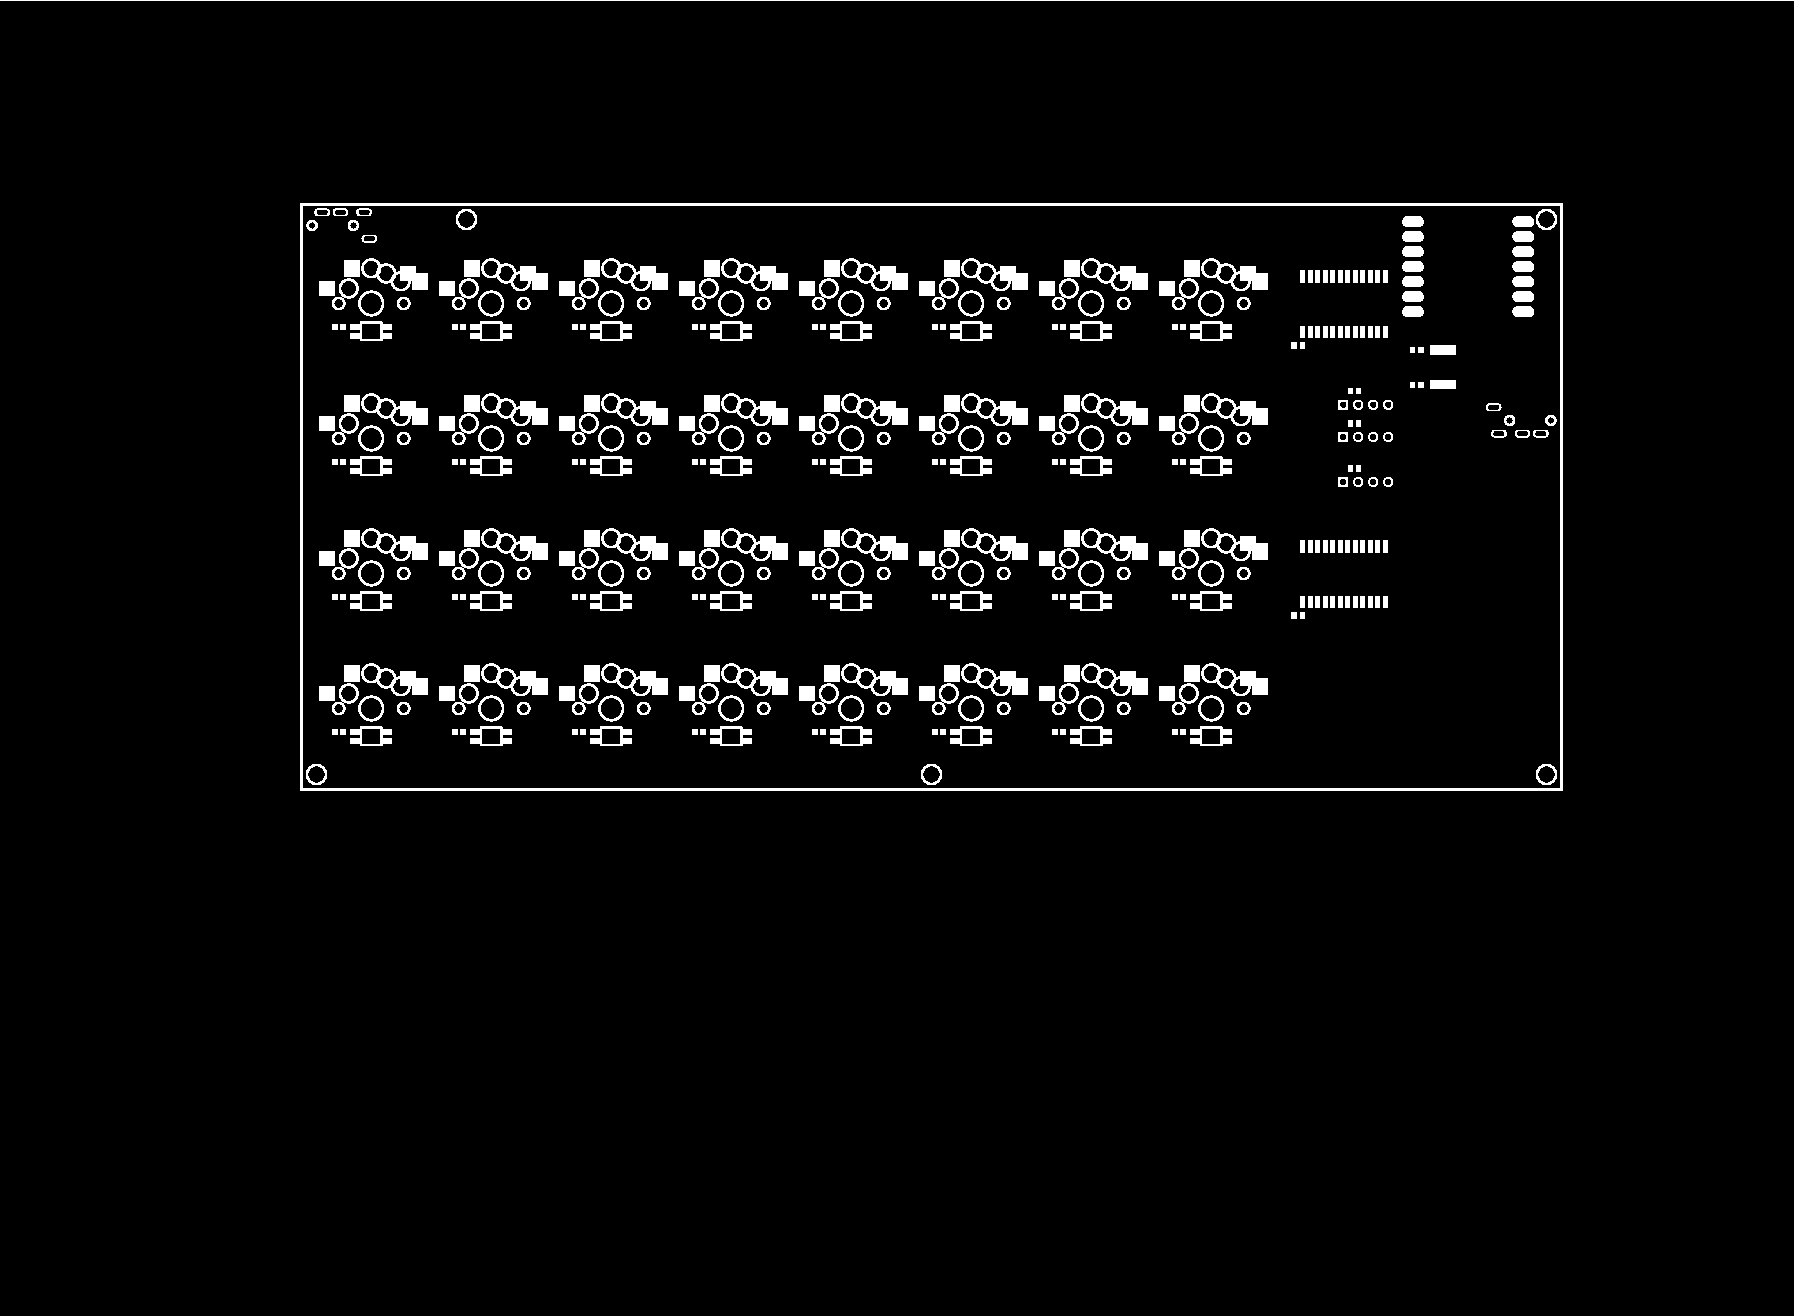
\includegraphics[width=0.9\textwidth]{Macruwu PCB_2}
		\caption{PCB frame 2 of the Macruwu}
	\end{figure}
	\begin{figure}[H]
		\centering
		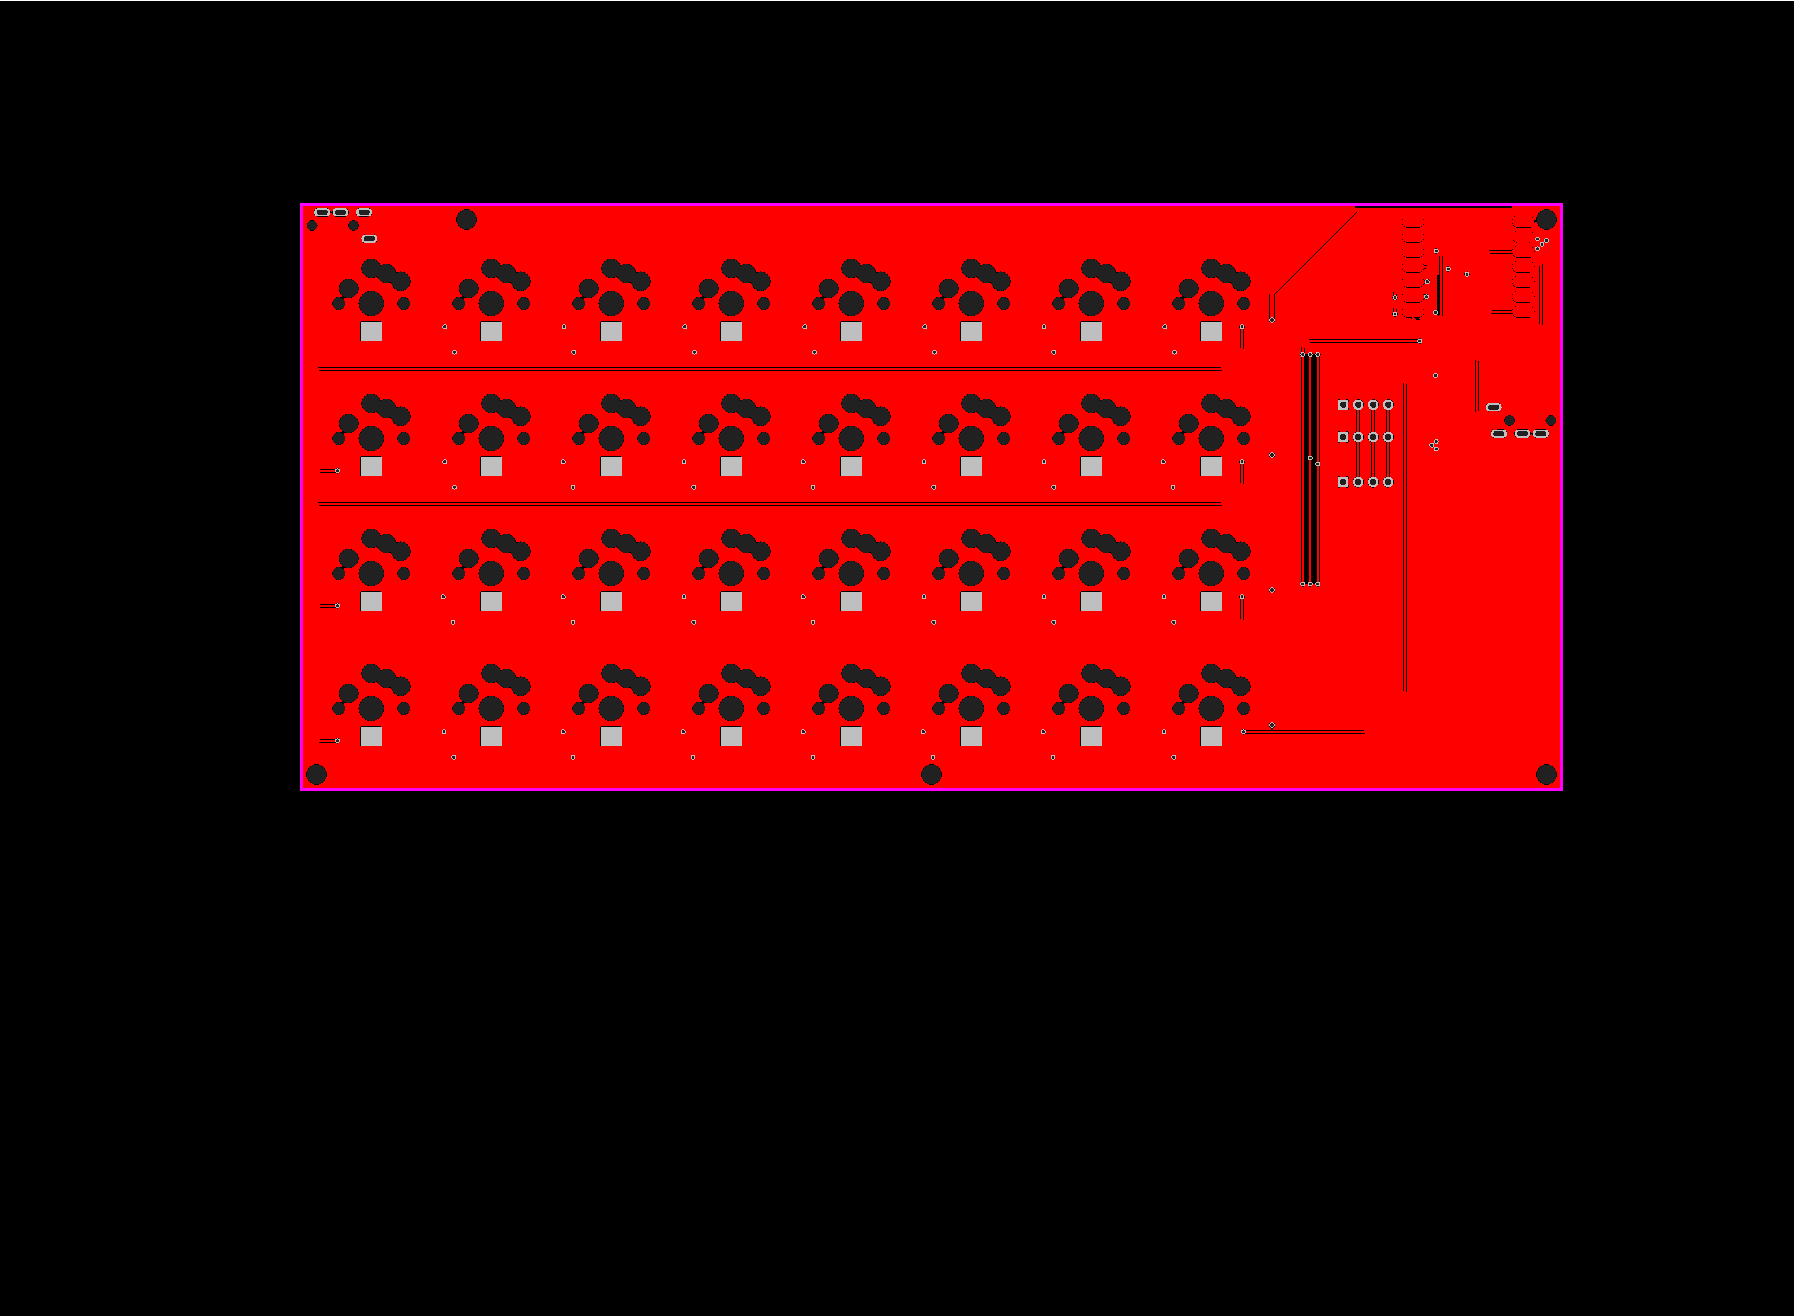
\includegraphics[width=0.9\textwidth]{Macruwu PCB_3}
		\caption{PCB frame 3 of the Macruwu}
	\end{figure}
	\begin{figure}[H]
		\centering
		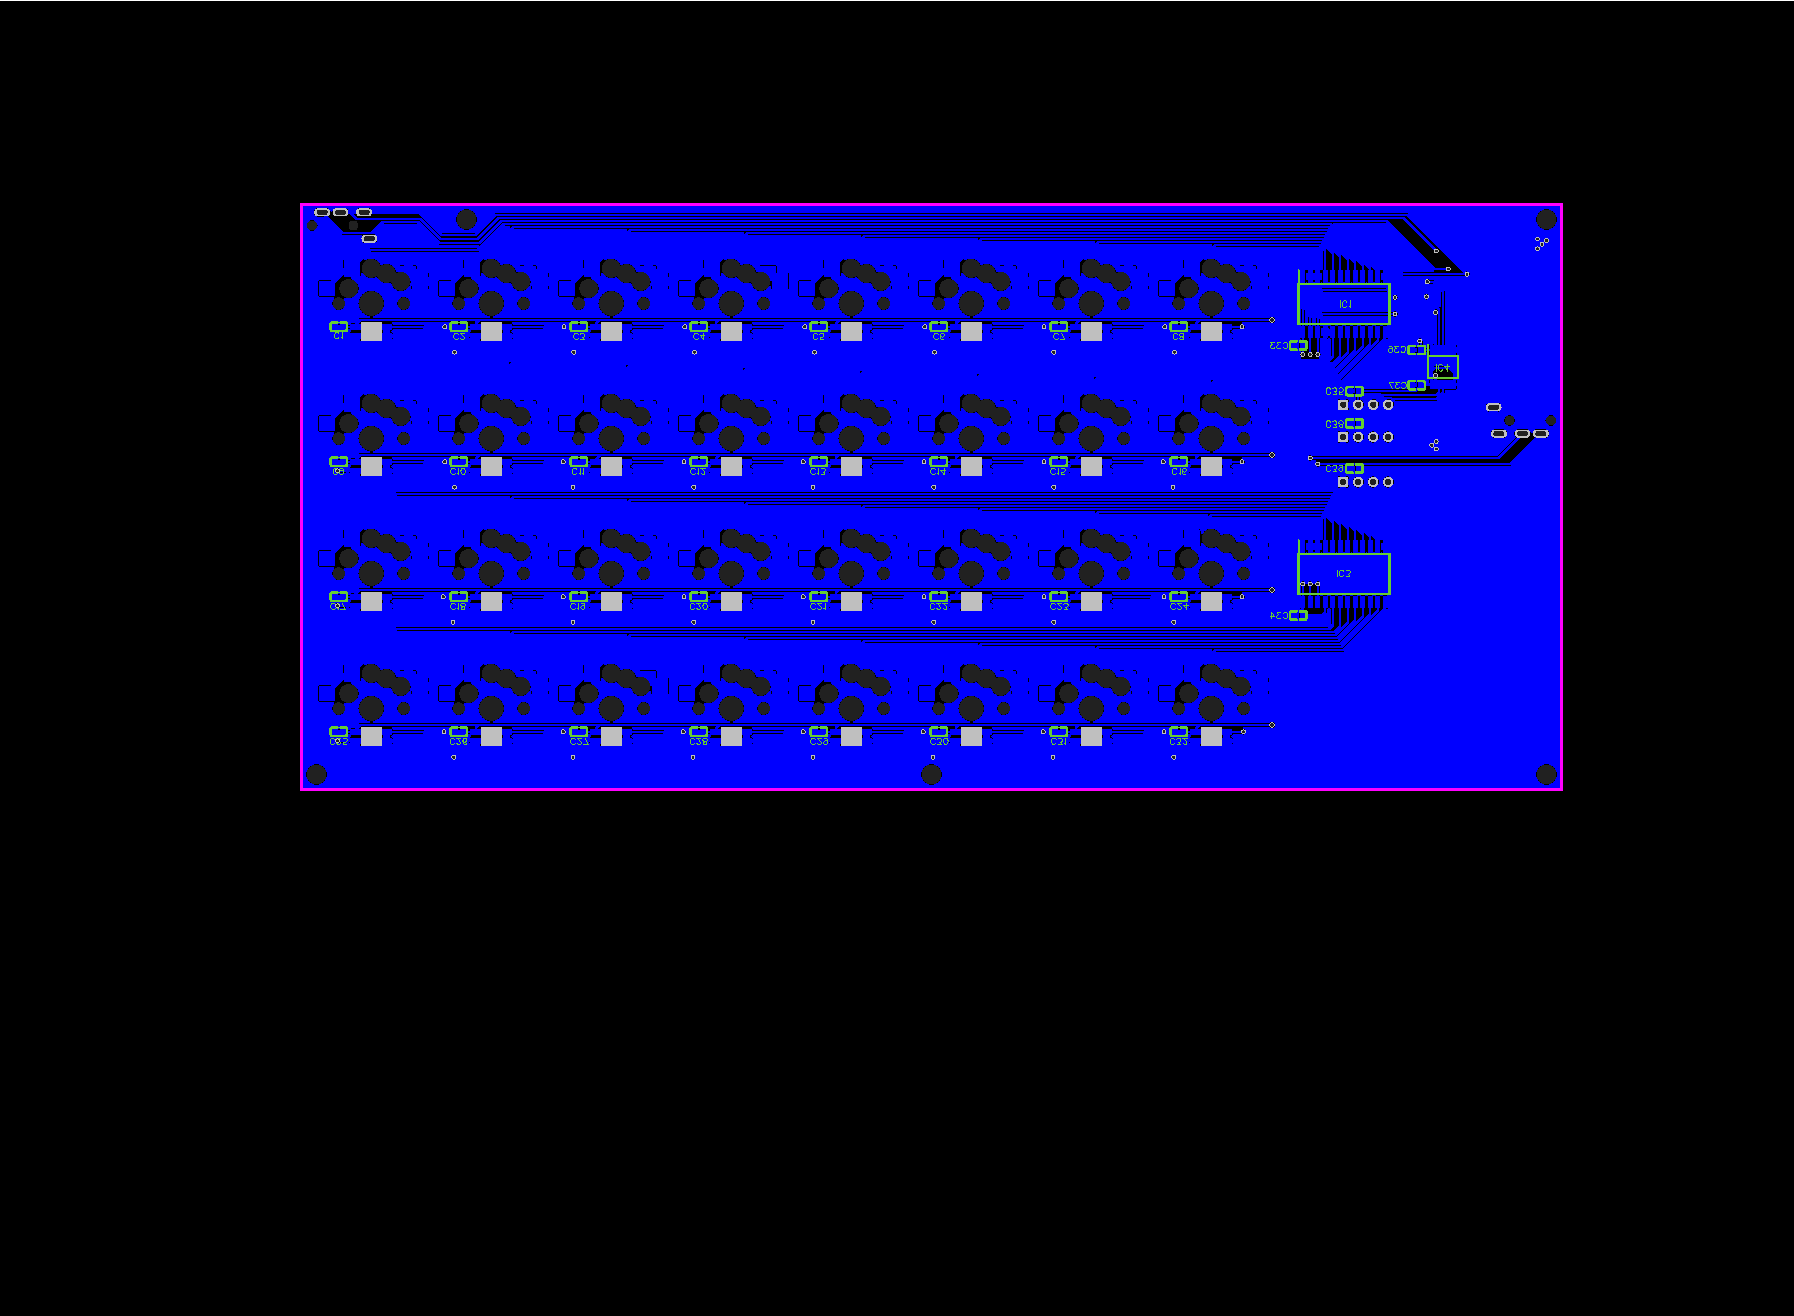
\includegraphics[width=0.9\textwidth]{Macruwu PCB_4}
		\caption{PCB frame 4 of the Macruwu}
	\end{figure}
	\begin{figure}[H]
		\centering
		\includegraphics[width=0.9\textwidth]{Macruwu PCB_5}
		\caption{PCB frame 5 of the Macruwu}
	\end{figure}
	
	\subsection{Soldering tips}
	SMD soldering is a pain, but in this case necessary. If you've never soldered SMD before or if it's been a while, here are some tips:
	\begin{itemize}
		\item Start with the smallest components. I'd recommend starting with the SMD capacitors. They're really fiddly, but are good for practice, especially if you haven't soldered SMD before. If you mess up, they're also easy to remove letting you try again. And if you manage to solder all the capacitors, the rest shouldn't be a problem.\newline
		\textbf{NOTE:} When soldering the capacitors, leave out the ones near the ICs and do them later. They might get in the way when soldering the ICs.
		\item When soldering the ICs, start by tinning a single pad. Once you've tinned one pad, heat it up and push the IC in to place. Then you can solder the rest of the connections.
		\item Use flux. It's not strictly necessary but it does help a lot, especially when using lead-free solder. If you find yourself getting a lot of bridges or cold solder joints, give flux a try. It really does help. I personally use the \href{https://www.amazon.de/FELDER-L%C3%B6tfett-L%C3%B6tmittel-Solder-L%C3%B6tpaste/dp/B01822CUO6}{flux paste you get in those small tins} but any flux is better than none.
		\item Have some solder wick lying around. If you find yourself unable to separate a bridge on an IC, you'll want solder wick. Ideally apply some flux to the wick, place it on the solder joints you want to disconnect and press your soldering iron on top. This should pull any unnecessary solder in to the wick.\newline
		\textbf{NOTE:} Don't pull the solder wick around the connection or PCB. This will scrape away the solder mask and may expose or cut traces. I found that out the hard way...
		\item When soldering in the hot-swap sockets and RGB LEDs, make sure they're properly soldered to the board. Ground pads especially tend to result in cold solder joints. Use flux and check your connections with a multimeter. For the hot-swap sockets you can increase the temperature to about 370-400°C, but try not to keep the iron on there for too long if you do. With the LEDs I'd recommend not going above 360°C because if you do, they might break. I haven´t had this happen before, but bear this in mind.
		\item Clean your board after soldering. You can use isopropanol or similar non conducting cleaning liquids. This is to prevent corrosion and general stickiness from the flux.
	\end{itemize}
	
	\section{Macruwu Firmware}
	This firmware is based on Earle Philhowers \href{https://github.com/earlephilhower/arduino-pico}{Arudino Pico} and includes some Adafruit libraries. Therefore, make sure to install them before trying to flash this code.
	\subsection{Structure}
	\textbf{NOTE:} I'm not studying computer science so this diagram may not be up to standard. However, I hope it gives you a brief overview of how the code is structured. This will be updated with code updates (hopefully).\newline
	\begin{minipage}{\linewidth}
		\centering
		\resizebox{0.5\textheight}{!}{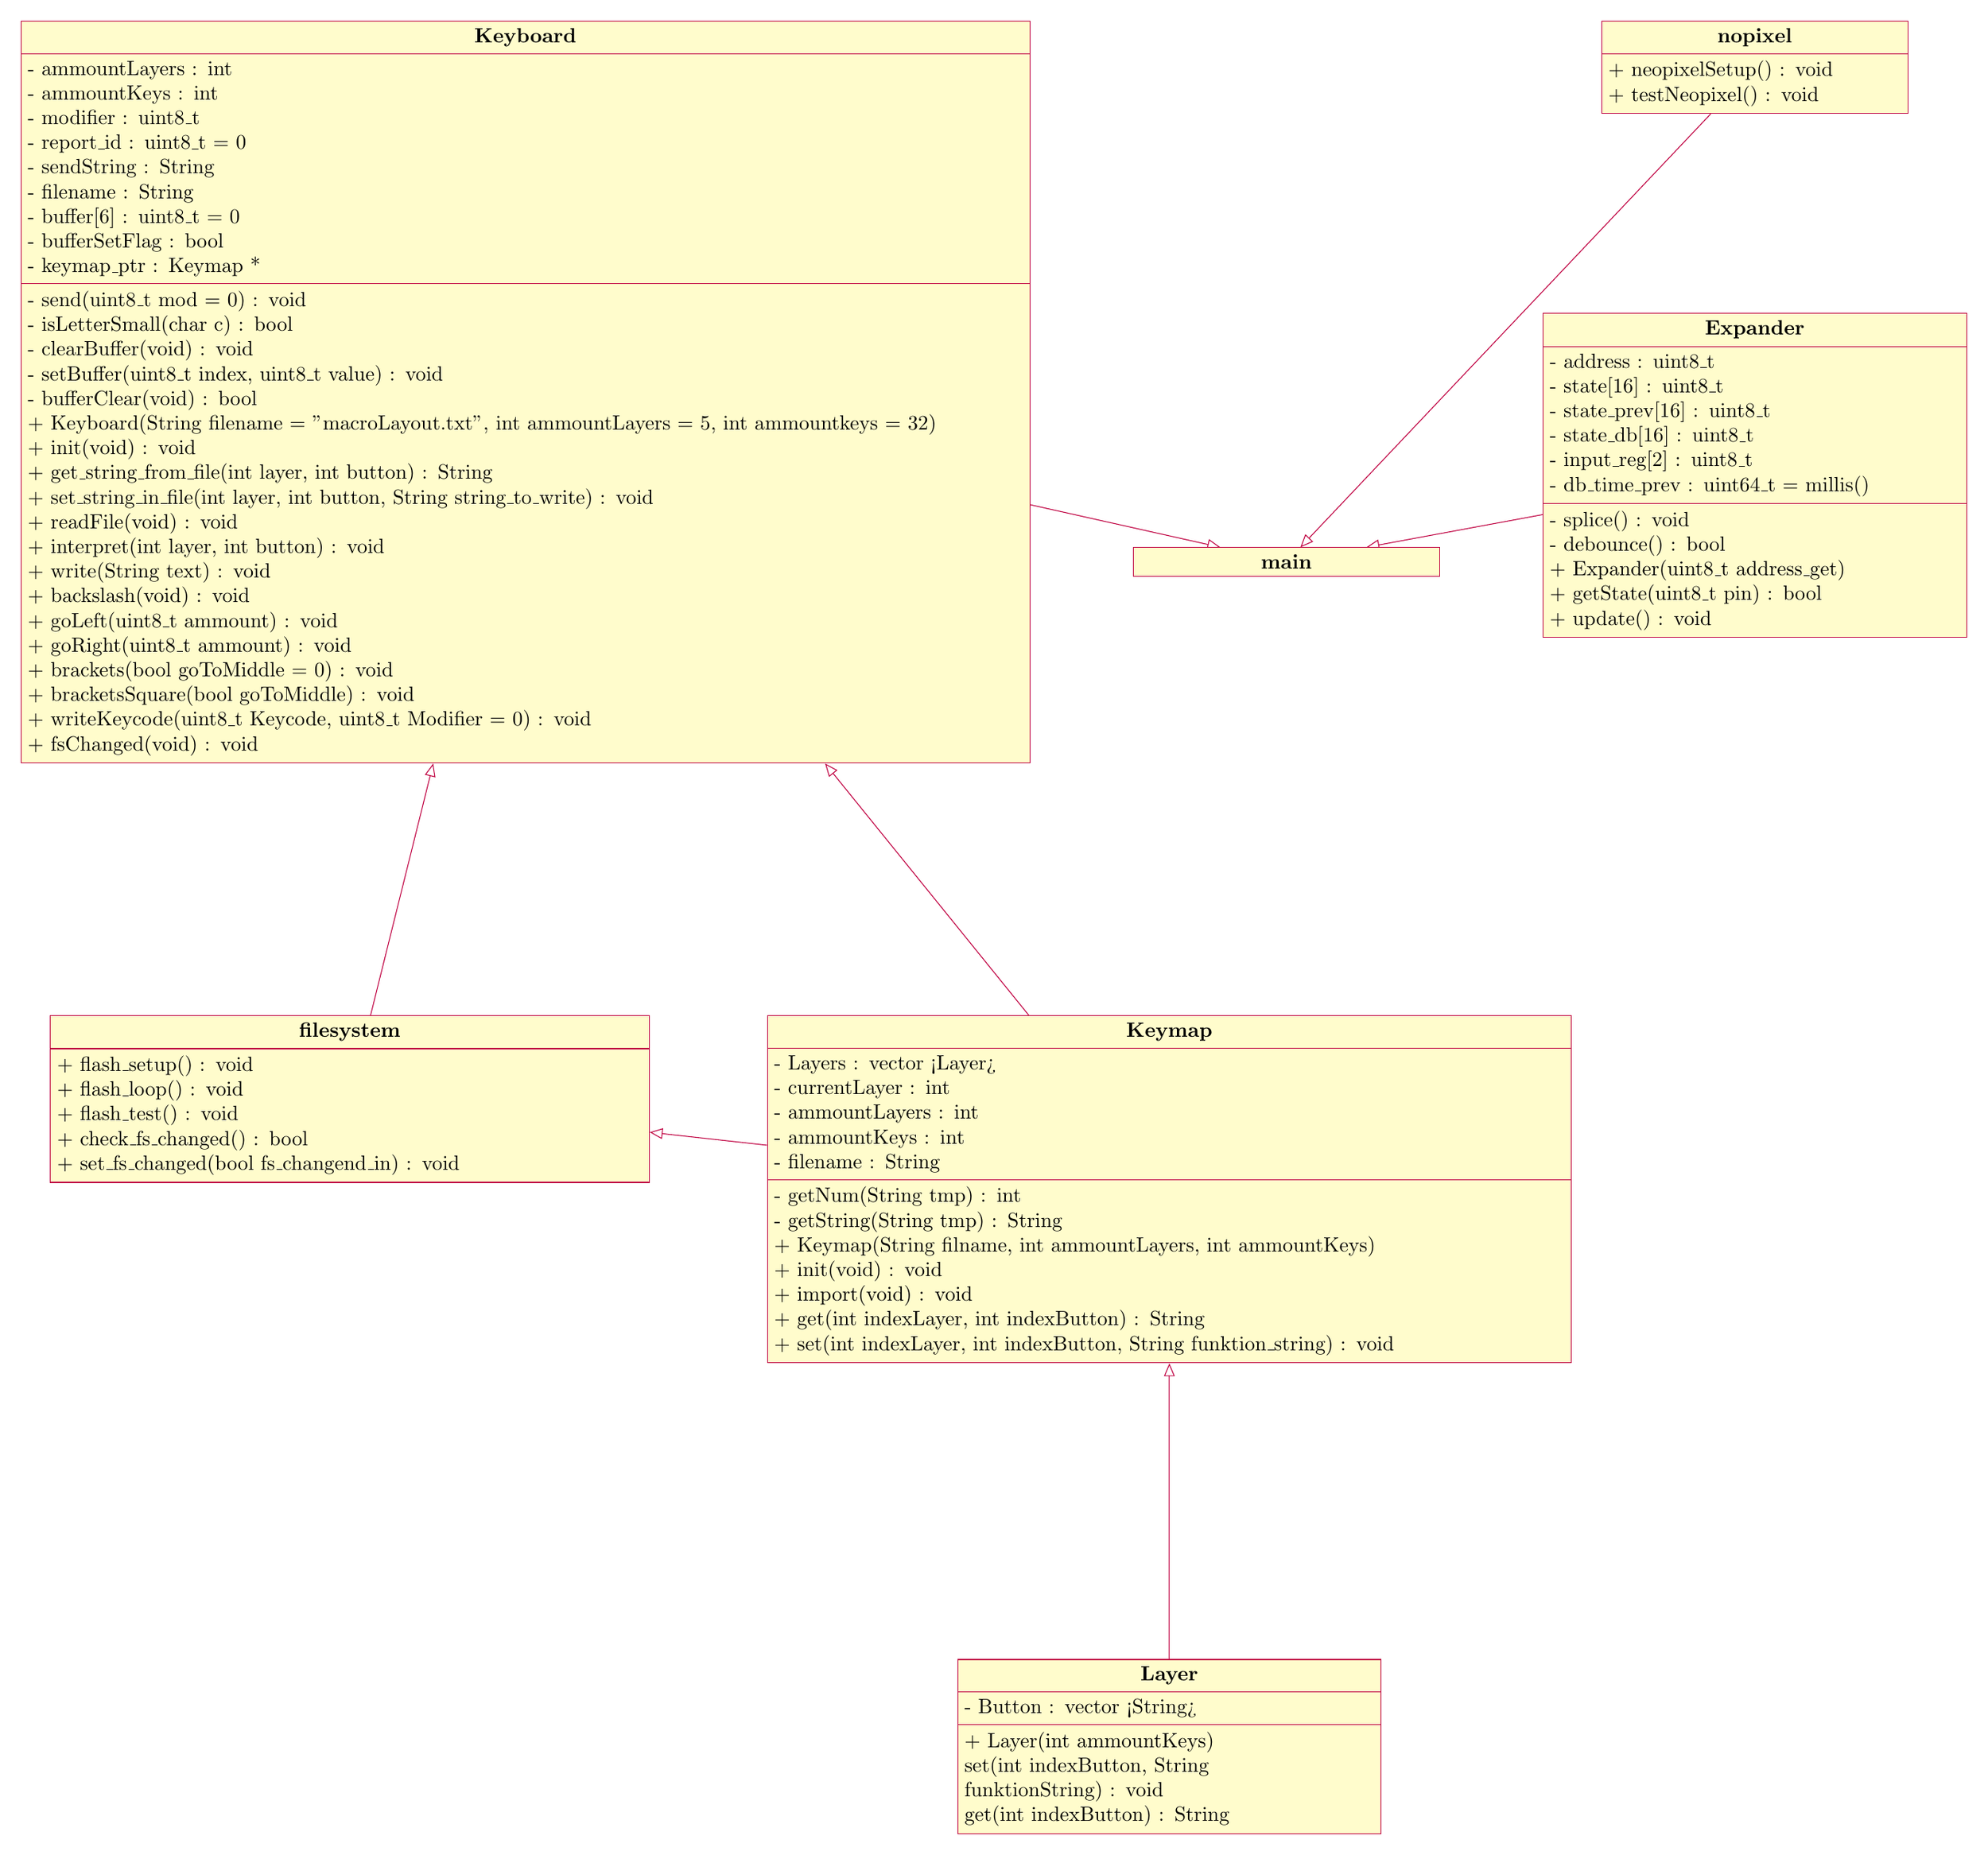
\begin{tikzpicture}
	\begin{class}{main}{9,-9}
	\end{class}
	
	\begin{class}[text width = 17cm]{Keyboard}{-4 ,0}
		\inherit{main}
		\attribute{- ammountLayers : int}
		\attribute{- ammountKeys : int}
		\attribute{- modifier : uint8\_t}
		\attribute{- report\_id : uint8\_t = 0}
		\attribute{- sendString : String}
		\attribute{- filename : String}
		\attribute{- buffer[6] : uint8\_t = {0}}
		\attribute{- bufferSetFlag : bool}
		\attribute{- keymap\_ptr : Keymap *}
		\operation{- send(uint8\_t mod = 0) : void}
		\operation{- isLetterSmall(char c) : bool}
		\operation{- clearBuffer(void) : void}
		\operation{- setBuffer(uint8\_t index, uint8\_t value) : void}
		\operation{- bufferClear(void) : bool}
		\operation{+ Keyboard(String filename = "macroLayout.txt", int ammountLayers = 5, 	int ammountkeys = 32)}
		\operation{+ init(void) : void}
		\operation{+ get\_string\_from\_file(int layer, int button) : String}
		\operation{+ set\_string\_in\_file(int layer, int button, String string\_to\_write) 	: void}
		\operation{+ readFile(void) : void}
		\operation{+ interpret(int layer, int button) : void}
		\operation{+ write(String text) : void}
		\operation{+ backslash(void) : void}
		\operation{+ goLeft(uint8\_t ammount) : void}
		\operation{+ goRight(uint8\_t ammount) : void}
		\operation{+ brackets(bool goToMiddle = 0) : void}
		\operation{+ bracketsSquare(bool goToMiddle) : void}
		\operation{+ writeKeycode(uint8\_t Keycode, uint8\_t Modifier = 0) : void}
		\operation{+ fsChanged(void) : void}
	\end{class}

	\begin{class}{nopixel}{17,0}
		\inherit{main}
		\operation{+ neopixelSetup() : void}	
		\operation{+ testNeopixel() : void}
	\end{class}
	
	\begin{class}[text width = 7cm]{Expander}{17,-5}
		\inherit{main}
		\attribute{- address : uint8\_t}
		\attribute{- state[16] : uint8\_t}
		\attribute{- state\_prev[16] : uint8\_t}
		\attribute{- state\_db[16] : uint8\_t}
		\attribute{- input\_reg[2] : uint8\_t}
		\attribute{- db\_time\_prev : uint64\_t = millis()}
		\operation{- splice() : void}
		\operation{- debounce() : bool}
		\operation{+ Expander(uint8\_t address\_get)}
		\operation{+ getState(uint8\_t pin) : bool}
		\operation{+ update() : void}
	\end{class}
	\begin{class}[text width = 10cm]{filesystem}{-7,-17}
		\inherit{Keyboard}
		\operation{+ flash\_setup() : void}
		\operation{+ flash\_loop() : void}
		\operation{+ flash\_test() : void}
		\operation{+ check\_fs\_changed() : bool}
		\operation{+ set\_fs\_changed(bool fs\_changend\_in) : void}
	\end{class}

	\begin{class}[text width = 13.5cm]{Keymap}{7,-17}
		\inherit{Keyboard}
		\inherit{filesystem}
		\attribute{- Layers : vector <Layer>}
		\attribute{- currentLayer : int}
		\attribute{- ammountLayers : int}
		\attribute{- ammountKeys : int}
		\attribute{- filename : String}
		\operation{- getNum(String tmp) : int}
		\operation{- getString(String tmp) : String}
		\operation{+ Keymap(String filname, int ammountLayers, int ammountKeys)}
		\operation{+ init(void) : void}
		\operation{+ import(void) : void}
		\operation{+ get(int indexLayer, int indexButton) : String}
		\operation{+ set(int indexLayer, int indexButton, String funktion\_string) : void}
	\end{class}

	\begin{class}[text width = 7cm]{Layer}{7,-28}
		\inherit{Keymap}
		\attribute{- Button : vector <String>}
		\operation{+ Layer(int ammountKeys)}
		\operation{set(int indexButton, String funktionString) : void}
		\operation{get(int indexButton) : String}
	\end{class}
	
	
\end{tikzpicture}}
	\end{minipage}
	\newline
	\newline
	The basic idea of this code is to divide everything up in to separate modules that interface with one aother. This takes a bit more effort to try and get the separate modules working together, but once it's set up, it's a lot easier to tweak.
	\subsubsection{Layer class}
	OK, so now lets go over the structure and start at the bottom. The \textit{Layer} class has a vector of strings. This stores all the plaintext commands associated with a certain button. So a \textit{Layer}-object has several buttons.
	\subsubsection{Keymap class}
	The \textit{Keymap} class has a vector of \textit{Layer}-objects. A \textit{Keymap}-object thus has several layers consisting of several buttons. You can imagine this as an array or a table, that allows you to look up which command is associated with a certain button on a certain layer.
	\subsubsection{Filesystem' functions}
	The \textit{Keymap} class can also access the file system using the \textit{import()} method. This method pulls the command strings from the \textit{macroLayout.txt}-file stored on the internal file system and saves them in the aforementioned \textit{Layer-Button}-structure.
	\subsubsection{Keyboard class}
	This construct is then controlled by the \textit{Keyboard}-class. This builds an interface for the \textit{main} to access but also introduces some functions of its own. The \textit{Keyboard}-class manages all the HID(human interface device)-commands and also houses the interpreter to convert the command strings to sendable HID key-codes. This is done internally for the most part, but exposes all the relevant interface methods to the main. For example, the \textit{interpret(layer, button)}-method interprets and runs the command stored in the command string at the given layer and button as an HID command.\newline
	\textbf{NOTE:} All HID commands are set to work with a German keyboard layout. Most of them still work with a US or similar layout, but you might have to change some special character keycodes like '\verb=^=' or '\verb=\='.\newline
	Edit: I found a overview of a keyboard with the corresponding key-codes depicted on every key. This should be universal to all Keyboards. May be useful...
	\begin{figure}[H]
		\centering
		\includegraphics[width=0.9\textwidth]{HIDkeys}
		\caption{Mapped HID Keys}
	\end{figure}
	
	\noindent There are also other methods included in the class. The \textit{readFile()}-method in combination with the \textit{fsChanged()}-method can auto-update the \textit{Layer-Button}-structure from the \textit{macroLayout.txt}-file whenever the file is edited.
	\subsubsection{NoePixel functions}
	So far not a lot has been done here. These are just a few function prototypes saved in a separate file. \textit{neopixelSetup()} simply initialises the Adafruit library and \textit{testNeopixel()} just runs a slow rainbow-effect.
	\subsubsection{Expander class}
	The \textit{Expander}-class is responsible for reading and debouncing the I/O expanders. The state of any pin on the I/O expander can be accessed via the \textit{getState} method.
	\subsubsection{Mapping module}
	This isn't shown in the diagram and is mainly for debugging and testing. The \textit{Mapping} module is a header and source file combination that creates its own \textit{Keyboard}-object and runs hardcoded sets of instructions when a button is pressed. The function of a certain button can be called from the main via the \textit{action(button)}-function.
	\subsection{AniMacro}
	The AniMacro scripting language (kinda) is used to tell the macropad what to type from the \textit{macroLayout.txt}. This is fully customisable and you can add your own commands in the \textit{Keyboard::interpret()} method if you are so inclined.\\
	The basic structure, however, is set by the \textit{readFile()}-method. With \textit{Layer x:} you set the current layer to x. Follow that with \textit{Button y: something} and you set button \textit{y} on layer \textit{x} to \textit{something}. Every \textit{Layer x:} or \textit{Button y: something} must be followed by a linebreak.\newline
	\textbf{For example:}\newline
	\noindent\fbox{%
		\parbox{\textwidth}{%
			\begin{tabbing}
				Layer 1:\= \\
				\> Button 1: something \\
				\> Button 2: something else \\
				Layer 2:\\
				\> Button 1: something on Layer 2
			\end{tabbing}
		}%
	}\newline
	\subsubsection{Implemented commands}
	\begin{tabular}{|l|m{6.5cm}|m{6.5cm}}
		\hline
		\textbf{Command} & \textbf{Description} & \textbf{Comment}\\
		\hline
		\hline
		\verb=Some text= & No operator prints plain text& \\
		\hline
		\verb=\plain{}= & Prints contents as plain text. Can print characters reserved for AniMacro commands. & Double Brackets \verb={}= will be printed. If the have contents (e.g. \verb={a}=), the plain command chain is broken and returned to the 'no Operator' state.\\
		\hline 
		\verb=<= & Moves screen cursor one step to the left (presses left arrow key) & \\
		\verb=>= & Moves screen cursor one step to the right (presses right arrow key) & \\
		\verb=\n= & Triggers the 'ENTER'-key & \\
		\verb=\t= & Triggers the 'TAB'-key & \\
		\hline
	\end{tabular}\\\\
	Most special characters can also be typed without a special command:\\
	\verb=\ ^ { } [ ] ( ) $ | _ . ,=
	
	\subsection{I$^2$C Expansion Port}
	\noindent
	The I$^2$C expansion port is used to connect peripherals to the Macruwu via a TRRS-jack. It can also be used to connect the Macruwu as a peripheral to another Macruwu. The Pins are as follows:
	\begin{center}
		\begin{tabular}{|c|c|c|c|}
			\hline
			Sleve&Ring 1& Ring 2& Tip\\
			\hline
			GND & SCL 3V3 & SDA 3V3 & 5V\\
			\hline
		\end{tabular}
	\end{center}
	The Macruwu connected to USB is always the main master, so connected devices must be configured as Slaves. However the RP2040 offers a second I²C Port, wich can be configured a slave, so you can daisychain several Macruwus.
	\subsubsection{I²C Structure}
	\textbf{Write:}\\
	\begin{tabular}{|c|c|c|c|c|c|c|c|c|c|c|}
		\hline
		S&Address&1&A&Register/Command&1&A&Data(8-bit)&A&...&E\\
		\hline
	\end{tabular}
	\\\\
	\noindent\textbf{Read:}\\
	\begin{tabular}{|c|c|c|c|c|c|c|c|c|c|c|c|c|c|}
		\hline
		S&Address&1&A&Register/Command&E&S&Address&0&A&Data(8-bit)&A&...&E\\
		\hline
	\end{tabular}
	\\\\
	\textbf{S}: START\\
	\textbf{E}: STOP/END\\
	\textbf{A}: ACK\\
	\\
	\noindent The default Address is 0010 101 and 7-bit wide.
	\subsubsection{Registers/Commands}
	\begin{center}
		\begin{tabular}{|m{0.25\linewidth}|m{0.15\linewidth}|m{0.6\linewidth}|}
			\hline
			Register/Command&Mode&Description\\
			\hline
			0000 0000(0x00)&Read&Get Button Layout config. This will send over The amount of Keys and other Important Information elaborated on in \ref*{Config}.\\
			\hline
			0000 0010(0x02)&Read&Get Inputs. This will return the State on Buttons pressed as a multiple of 8-bit Registers.\\
			\hline
			0000 0100(0x04)&Read&Get Keycodes. This will send Keycodes, modifiers and the Report IDs as 3-byte blocks.\\
			\hline
			0000 0101(0x05)&Write&Send Keycodes. Used for the Bluetooth expansion header to send the parsed Keycodes to the Bluetooth Board.\\
			\hline
			0000 0110(0x06)&Read&Get string to print: This will return a string that can be interpreted by the host Macruwu.\\
			\hline
			0000 0111(0x07)&Write&Send String as a C-String (character array).Used for Bluetooth expansion board if set to Interpreter Mode\\
			\hline
			0100 0000(0x40)&Reserved&Address of I/O Expander. Would cause confusion...\\
			\hline
			0100 0001(0x41)&Reserved&Address of I/O Expander. Would cause confusion...\\
			\hline
			0110 1001(0x69)&Reserved&Address of Bluetooth Module. Would distract the boys...\\
			\hline
		\end{tabular}
	\end{center}
	\subsubsection{Configuration}
	\label{Config}
	\begin{center}
		\begin{tabular}{|m{0.2\linewidth}|m{0.2\linewidth}|m{0.6\linewidth}|}
			\hline
			Data type&Variable&Description\\
			\hline
			\verb=uint8_t=&\verb=ammount_keys=&Key count registered to the expansion device. If this is not used send 0000 0000(0x00)\\
			\hline
			\verb=uint8_t=&\verb=language_set=&Keyboard language set on host. Can be used to set the ASCII to keycode Table in expansion Modules with keycode sending functions. If this is not used send 0000 0000(0x00)\\
			\hline
		\end{tabular}
	\end{center}

	\subsection{Language Codes}
	\begin{center}
		\begin{tabular}{|m{0.2\linewidth}|m{0.2\linewidth}|m{0.6\linewidth}|}
			\hline
			Language Code&Value&Comment\\
			\hline
			GERMAN&0000 0000(0x00)&DEFAULT\\
			\hline
			\verb=ENGLISH_US=&0000 0001(0x01)&\\
			\hline
		\end{tabular}
	\end{center}

	\section{Debugging tips}
	\begin{figure}[H]
		\centering
		\includegraphics[width=0.9\textwidth]{debugging}
		\caption{Debugging tips from the IT crowd}
	\end{figure}
	Sometimes the Macruwu gets stuck and cant get out (of an infinite loop or something). Unplugging it and plugging it back in again can help with that and works in 90\% of all cases.\\
	If this does not help, try the tips below.
	\subsection{Compiling firmware}
	\begin{itemize}
		\item Check whether you have the correct version of the Arduino Pico framework installed. I used the newest at the time, which was version 2.6.4.
		\item Also check, that you have the correct libraries installed.
		\subitem Adafruit NeoPixel by Adafruit (1.10.6)
		\subitem Adafruit SPIFlash by Adafruit (4.0.0)
		\subitem SdFat - Adafruit Fork by Bill Greiman (2.2.1)
		\item If you are using Platform I/O or similar, you may have to include files other than the main separately in the compiler config
	\end{itemize}
	\subsection{Microcontroller crashing}
	\begin{itemize}
		\item Try running the \textit{flash\_test()} function in the setup. This will create the \textit{macroLayout.txt} which if missing might cause the microcontroller to crash.
		\item If the microcontroller doesn't get recognised by the computer, try holding down the \textit{BOOT}-button on the microcontroller and while pressing it, plug the microcontroller back in to the computer. It will them show up as a new device, and COM port and you should be able to upload to it.
	\end{itemize}
	\subsection{Filesystem corrupted}
	This can happen, if the \textit{File read} protocol crashed, due to a illegal character in the \textit{macroLayout.txt} file on the flash. If this happens, please open a issue with the character, that caused the crash.\\
	There is a way to 'restore' it though.
	\begin{enumerate}
		\item Unplug the Macruwu and uncomment the \textit{flash\_clear()} command. This will clear the flash partition.
		\item Hold the \textit{BOOT} button (the on on the right) on the RP2040 and plug it in while pressing the button. This will manually set the microcontroller in to programming mode.
		\item Select the newly appeared COM port and press upload. You may have to restart the Arduino IDE several times throughout this process, if it is stuck in a infinite upload loop. Don´t worry, this will not break anything.
		\item Once uploaded, a new drive should show up. If you are under Windows you will be prompted to format the disc.
		\item Once formatted, you can upload a backup of the \textit{macroLayout.txt} or create a new one. DO NOT UNPLUG THE MACRUWU!
		\item Go to the Arduino IDE and comment or delete the \textit{flash\_clear()} command.
		\item Select the correct COM port and press upload. If the Arduino IDE is stuck in a infinite upload loop, restart the IDE. 
		\item It should be working normally again.
	\end{enumerate}
	\subsection{NeoPixels not working}
	\begin{itemize}
		\item Check the solder connections. If the NeoPixels are not properly soldered on to the pads they will not work. Even one improperly soldered NeoPixel may cause the others to act funny. I recommend checking each connection with a multimeter, by connecting one probe to $GND$ or $5V$ respectively and going through the respective pins on the NeoPixels with the other.
		\item If $5V$ and $GND$ are connected correctly, but you are still having trouble, check the connection between the Neopixels. $D_{out}$ of one and $D_{in}$ of the next in the chain should always be connected.
	\end{itemize}
	\subsection{I/O expanders not working}
	\begin{itemize}
		\item Check the solder connections
		\item Make sure your I/O Expanders have internal pull-up resistors. If they do not, they will not work with the Macruwu board. If you have your own board, you can also add them on the PCB, however, I did not do that with mine.
		\item Make sure you have set the correct address. The Base address can be found in the datasheet of the I/O expander and the variable address pars can be found in the Macruwu schematic. If you are using the same I/O listed in the materials section, the preset address should be correct.
		\item If you are using different I/O expanders from the ones listed in the materials section, make sure the I$^2$C addressing scheme is correct. Other I/O expanders may need to be configured differently from the ones I used. If it turns out that you do need a setup sequence for your I/O expanders, you can create a \textit{init()} method in the \textit{Expander} class and call it in the \textit{setup()}.
	\end{itemize}
	\subsection{some buttons are not being recognised}
	\begin{itemize}
		\item Check the solder connections on the hot-swap sockets. They tend to form cold solder joints, that you may not always see. Especially the GND pad tends to do this. Check the connection with a multimeter by holding one probe to a known GND and going through the other connections with the other probe. The same can be done for the other side of the socket. Hold one probe on the socket and the other on the corresponding I/O expander pin.
		\item Make sure the key switch is installed correctly. The pins do tend to bend when pressing them in. you can check from the underside of the board, if the pin is seated in the hot-swap socket. If not, pull it out, straighten out the pin with a pair of pliers and press it back in.
	\end{itemize}
	If none of the above helped, fell free to contact me.\\
	Discord: Bramble\#2342
\end{document}